\section{Coral Dev-Board}
\label{sec:hard-devboard}
The Coral Dev Board is a single-board computer that contains an Edge TPU
coprocessor. It's ideal for prototyping new projects that demand fast on-device
inferencing for machine learning models.
%
\begin{figure}[htb]
	\centering
    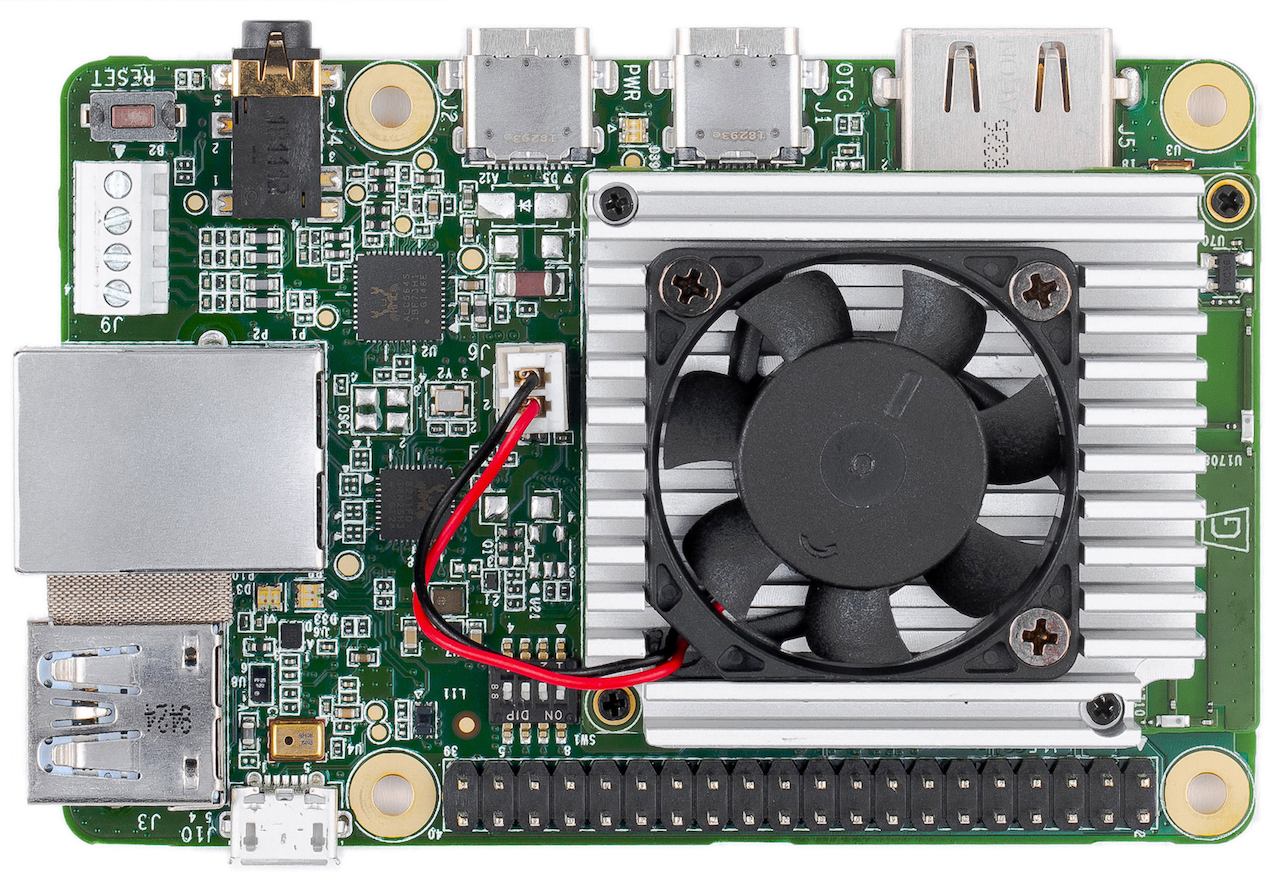
\includegraphics[width=0.80\textwidth]{devboard-dimensions.jpg}
    \captionsource{Coral Dev Board.}{
    \href{https://coral.ai/docs/dev-board/get-started/}{https://coral.ai/docs/dev-board/get-started/}}
    \label{fig:boardcam}
\end{figure}
%
\subsection{Overview}
\label{ssec:hard-devboard-overview}
The Coral Dev Board is a single-board computer that's ideal when you need to
perform fast machine learning (ML) inferencing in a small form factor. You can
use the Dev Board to prototype your embedded system and then scale to production
using the on-board Coral System-on-Module (SoM) combined with your custom PCB
hardware. The SoM provides a fully-integrated system, including NXP's iMX 8M
system-on-chip (SoC), eMMC memory, LPDDR4 RAM, Wi-Fi, and Bluetooth, but its
unique power comes from Google's Edge TPU coprocessor. The Edge TPU is a small
ASIC designed by Google that provides high performance ML inferencing with a low
power cost. For example, it can execute state-of-the-art mobile vision models
such as MobileNet v2 at almost 400 FPS, in a power efficient manner. 
The baseboard provides all the peripheral connections you need to prototype a
project, including USB 2.0/3.0 ports, DSI display interface, CSI-2 camera
interface, Ethernet port, speaker terminals, and a 40-pin I/O header. \hfill \break
Key benefits of the Dev Board:
\begin{itemize}
	\item High-speed and low-power ML inferencing (4 TOPS @ 2 \si{\watt})
	\item A complete Linux system (running Mendel, a Debian derivative)
	\item Prototyping and evaluation board for the small Coral SoM (40 x 48 \si{\milli\meter})
\end{itemize}



\begin{table}[htb]
	\centering
	\begin{tabular}{c}
	\hline \\
Edge TPU System-on-Module (SoM)\\
% NXP i.MX 8M SoC (Quad-core Arm Cortex-A53, plus Cortex-M4F)
% Google Edge TPU ML accelerator coprocessor
% Cryptographic coprocessor
% Wi-Fi 2x2 MIMO (802.11b/g/n/ac 2.4/5 GHz)
% Bluetooth 4.2
% 8 GB eMMC
% 1 GB LPDDR4
% USB connections
% USB Type-C power port (5 V DC)
% USB 3.0 Type-C OTG port
% USB 3.0 Type-A host port
% USB 2.0 Micro-B serial console port
% Audio connections
% 3.5 mm audio jack (CTIA compliant)
% Digital PDM microphone (x2)
% 2.54 mm 4-pin terminal for stereo speakers
% Video connections
% HDMI 2.0a (full size)
% 39-pin FFC connector for MIPI DSI display (4-lane)
% 24-pin FFC connector for MIPI CSI-2 camera (4-lane)
% MicroSD card slot
% Gigabit Ethernet port
% 40-pin GPIO expansion header
% Supports Mendel Linux (derivative of Debian)
\hline
	\end{tabular}
	\caption{Coral Dev Board Features.}
	\label{tab:hard-devboard-spec}
\end{table}

Google Colar accelerator are USB dongles with a special TPU chip performing all
tensor calculations The Google Coral works with special pre-compiled TensorFlow
Lite networks. If the topology of the neural network and its required operations
can be described in TensorFlow it may work well on the Google Coral. However,
with its sparse 1 Gbyte RAM, memory shortage can still be an issue. The Google
USB accelerator has its special back-end compiler converting a TensorFlow Lite
file to an executable model for the dongle TPU.
% reference https://qengineering.eu/deep-learning-with-raspberry-pi-and-alternatives.html#EfficientNet
%
\section{TPU explained in depth}
\label{sec:hard-tpu}
% cite page https://qengineering.eu/google-corals-tpu-explained.html

Introduction.
The Google Coral has a TPU on board which speeds up the tensor calculations enormously. These tensor calculations are used in deep learning and neural networks. How does such a Tensor Processing Unit work? On this page a thorough investigation.
Neural node.
Both the Google Coral Dev board and the Coral USB Accelerator use an ASIC made by the Google team called the Edge TPU. It is a much lighter version of the well-known TPUs used in Google's datacenter. It also consumes very little power, so it is ideal for small embedded systems. Nevertheless, the similarities in applied technology are significant. They both use a systolic array to do the tensor operations. First, let's start with neural nodes.

Neural networks used in deep learning consists of many neural nodes. They are all connected together in a defined way. The way these nodes are wired is called the topology of the network. This topology determines the function the network performs. See this list for a selection of several types of deep learning networks.
Each node has always three basic components. A multiplier multiplies all the inputs with their respective so-called weight, the synapses. An adder who accumulates all the individual multiplications. And an activation function that shapes the output given the addition. A schematic view below.

Neural network node

The formula can be written as follows.

Formula neuron

The bias is a constant that gives the network much greater flexibility. Mathematically it can be included in the mul-add summation by giving an extra input the value 1.0 and the associated weight the value of the bias. Below a three-layer neural network is shown. The corresponding algorithm of this network is easy to program; two nested for loops and you have your outputs. See the C code. It is all quite simple, no rocket science at all.
Three layer network
int j,i;
double sum;
//x[] inputs
//l[] hidden layer outputs
//y[] outputs
//Wl[][] weights hidden layer
//Wo[][] weights output layer
for(j=0;j<NoHiddenLayer;j++){
sum=0;
for(i=0;i<NoInput;i++){
sum+=x[i]*Wl[j][i];
}
sum+=1.0*Wh[j][i]; //the bias
l[j]=tanh(sum);
}
for(j=0;j<NoOutput;j++){
sum=0;
for(i=0;i<NoHiddenLayer;i++){
sum+=l[i]*Wo[j][i];
}
sum+=1.0*Wo[j][i]; //the bias
y[j]=tanh(sum);
}
There is one problem, the computing time. A deep learning network consists of millions of neural nodes distributed over many layers. Despite the simplicity of the code, only one multiplication and one addition, it still takes a lot of time to calculate all the intermediate layers and outputs. On a fast PC, it can take a few seconds. Keep also in mind that training a network requires thousands of epochs and it becomes obvious that it all takes far too much time to be practical.
  
Fortunately, the algorithm is well suited for parallel execution. If you want to calculate an intermediate value, say l0, you do not need to know the other values on the same layer (l1 to l14). All values are independent of each other.

A first step to speed up the algorithm could be to distribute the calculations over different cores if you have a multi-core CPU. In case of four cores, the first calculates W0 to W3, while core 2 simultaneously performs W4 to W7. At the same time generates core 3 W8 to W11 and core 4 calculates W12 to W14, given the example above. In theory, a reduction of the execution time of 75% is possible. However, programming is very difficult. It makes the network topology rigid and the transfer of values to and from the cores usually ends up in a bottleneck. All this leads to disappointing results.

By the way, distributing the algorithm over the processes and threads won't take you any further, since they are all time-sliced by the operating system. In other words, every process and their threads are placed after one and each other in time, each getting a little time frame (slice) to do their calculations before moving to the other thread or process.
 
A second option is the use of the Graphical Processing Unit, the GPU on a video card. These are made up with a lot of little parallel cores designed for very fast matrix calculations. You can read more about this topic here. The best choice is the use of the Tensor Processing Unit, the TPU. This device has been specially designed for the above neural node algorithm.
The adder.
When software is too slow, hardware is the answer. Let see how the Google's Edge TPU hardware is structured.
The three main components of the neural node, the multiplier, the adder and the activation function must be included in the hardware. Let start with the adder.
Below a schematic diagram of the hardware of a 4-bit adder. A and B are the inputs. If the output overflows C4 the carry out is set. C0 is the carry-in of a previous phase.

4 bit adder
 
Every basic digital gate (AND, OR, NOT) has its own symbol. They usually consist of two or three transistors. Signals A and B propagate through the circuit and generate the result A + B. Changing one of them alters almost immediately the output. This happens extremely very fast, within a few nanoseconds.
This so-called propagation time depends on the number of digital ports whose output changes. Sometimes two gates only change their state. Sometimes more the six gates in a chain must alter their output. The propagation time is therefore not fixed, but lies between two limits, a minimum and a maximum time, see diagram at the bottom of the drawing. By the way, al mentioned times are illustrative and have no relationship to any device.
Pipeline.
If the propagation time of one adder lies at 2 nSec, the maximum clock rate can be 500 MHz. As mentioned earlier, a neural node can have hundreds of inputs, all of which must be accumulated. Designing a chain of adders is not a technical problem. However, the propagation time increases dramatically. The last adder in the chain must wait for all intermediate results before its output becomes stable. With a chain of 250 inputs, each with a 2 nSec delay, the total time is now 500 nSec. Which gives a very slow clock of 2 MHz. The solution here is a pipeline structure. A memory element is placed after each adder that keeps the result stable for the next adder.

4 bit adder with register

The output of the registers is updated at the rising edge of the clock signal. That is the only time the output can change. When the clock signal is high or low or falls, the inputs cannot manipulate the output, it remains stable. Just before the clock rises, the input must be stable for a minimum time, also just after the rise. Here an illustrative 0.1 nS. The register has its own propagation time (0.4 nS). The total propagation for a new stable signal is now 2.5 nS, which results in a maximum clock speed of 400 MHz. When placing the adders after each, you get the following situation.

Digital pipeline.

  
Each color represents a value. After four clock cycles, the value at the input has propagated through the network and appears at the output. Because the registers are updated simultaneously a new input is accepted every 2.5 nS.  The propagation time has been restored. The time it takes to travel through the whole pipeline is called latency time and is 10 nS in the above diagram (4 x 2.5nS). This pipeline technology is the backbone of modern computer technology and can be found everywhere. Every digital component is built on large pipelines which guarantee the required speed.  
The mul-add cell.
Every input signal of the neural node has its own effect on the final result. This gives one simple multiplication per input with a weight value. Just like an adder, a multiplication can build with the same basic digital gates. As you can imagine, more gates are now needed to perform a multiplication than a summation. In the formula of the neural node, each input is multiplied by its own weight value. The symbol can therefore even more straightforward.

Mul-Add register

  
For the sake of simplicity, no additional propagation time fixing registers have been added.
With the formula of the neural node in mind, it is now relatively easy to design such a neuron with a few mul-add cells. Below the schematic for a three input neuron.

3 input neuron

  
One important point to mention, are the registers at input X1 and X2. They create a delay line and are placed here to synchronize the necessary latency in the mul-add chain. When the second mul-add cell accumulates the output from the first cell (signal A) it is delayed one clock cycle. Therefore the multiplication of X1 with its weight need also be delayed one cycle in order to have the results at the same time. The color scheme above the design makes it all clear. Every color is now an element of the input vector [X0, X1, X2]. Looking at the horizontal lines, inputs A and B have always identical colors. Meaning they appear simultaneous, they are synchronized. The same applies to inputs C and D.
Systolic array.
Once a neural node has been created, it is easy to extend this scheme for the other neurons on the same layer. Given that each individual input is connected to all neurons in the next layer, the diagram will look like this.
Systolic Array Edge TPU
This type of design is called a systolic array. All values are pumped through the stages from top to bottom, hence the name. Looking at the timing, the array can accept a complete input vector every clock cycle. So, the propagation is still intact with 2.5 nS in the above-mentioned examples. At the same speed, the array generates complete output vectors. If the systolic array expands in depth or width, the propagation time still remains the same. Only the latency time increases. This enormous parallel calculation capacity is the reason why systolic arrays are widely used in neural network hardware.
 
The sizes of the systolic array in the Edge TPU are not known yet. The first TPU Google uses in its datacenter contains 256 x 256 mul-add cells. Running at 700 MHz it can theoretical performs 256 x 256 x 700.000.000 = 46 trillion mul-adds per second. Or if you look to individual operations 92 trillion (92 TOPS). However, this impressive figure is purely theoretical. In practice, there are some factors that slow performance.
 
The systolic array is made up of hardware. This means that it has fixed dimensions. Therefore, the input and output vectors also have fixed dimensions. However, the numbers of neurons per layer are determined by the design and are certainly not constant. If the number is smaller than the size of the array, it is, of course, possible to expand an input vector with leading zeros, so that the dimension equals the array size. The same technique can be applied to an oversized output vector.

If the input vector contains more elements than the width of the systolic array, the entire arithmetic calculation must be performed in more than one call. To this end, the input vector is cut into a series of smaller vectors that match the width of the series. They are then processed one after the other. The intermediate results must be stored in a buffer. These values must be added after completion of all the systolic calls.
Note that not only the input vector is split into smaller parts, but all weights used in the multiplication must be updated according to the formula's processing section. This may require a massive memory transfer. Below an example of a systolic array with only four inputs processing a vector of size 12.

Systolic formula

Looking at Google's schematic overview of the TPU, these output buffers and accumulators are drawn at the bottom. (In their diagram, the output is at the bottom instead of the right as on our drawing).  
Google TPU detail

  
Buffers have also been placed on the input vector side in the diagram above. They act as a first-in-first-out buffer, a FIFO. This guarantees continuous input of the systolic array with input values. It may also have some rotating operations, which increases the performance of CNN networks. It is unclear whether Google uses this method here.  
Activation unit.
Once the output is available, it is sent to the activation unit. This module within the Edge TPU applies the activation function to the output. It is hardwired. In other words, you cannot alter the function, it works like a ROM. Probably it is a ReLU function as it is nowadays the most used activation function and it is very easy to implement in hardware.  
TPU versus Edge TPU.
The Google's Edge TPU is a much smaller device than the TPUs that Google uses in its data centers. Below the PCB with the original TPU and the Edge TPU on the same scale.
TPU vs Edge TPU
It is obvious that such a small device cannot have the same functions as its much larger ancestor. The floor plan on the die does not allow this to happen. Nor can the systolic array have the 256 x 256 dimension as in the original TPU. Google has so far not revealed the measures in the Edge, but a well-founded estimate is 64 x 64 with a clock of 480 MHz, resulting in 4 TOPS.
Memory is also an issue. In the original chip, it takes around 29% of the total floor plan. It is impossible that the same amount can be found on the Edge TPU die. Moreover, the chip is very energy efficient. It requires no cooling. This means that almost certainly all the buffering is outside the chip. It leaves only a simple transfer of input vectors, output vectors and weights to the chip.  
Practice.
In fact, that is the whole concept of the Google Coral Dev board. Transfer all tensor calculations to the TPU as quickly as possible, fetch for the results, fill them in the next layer and start the cycle again with this layer. Process all layers one by one until they are ready.
To speed up the process, TensorFlow uses a special back end compiler, the Edge TPU compiler. The main task of this Edge TPU compiler is to partition the TensorFlow Lite file into more suitable TPU transfer packages. If for any reason the TPU cannot process the TensorFlow Lite file or part of it, the CPU will take care of it. However, if this happens, your application will, of course, work extremely slowly.
8 bits integers.
Another way of speeding up the calculations is the use of 8 bit signed integers instead of floats. A floating number occupies 32 bits in memory whereas the integer only needs 8. Because a neural network is fairly insensitive to number accuracy, it will also work well with 8-bit integers. It will still remain accurate. Not only does this technology save approximately 75% memory, but it also significantly reduces the number of transistors on the chip. If you look at the adder at the top of the page, you can imagine how many transistors a floating-point adder needs. Without this compression, the Edge TPU would not be as powerful, small and energy efficient.

The converting algorithm from floating point to 8 bit signed integer is quite simple. First, it determines which maximum and minimum a variable will take in the model. The larger of the two is then taken and scaled to 127. Suppose minimum is -1205.8 and maximum is 646.8. The larger is the min value of 1205.8. So that number becomes -127. Zero remains zero. That gives 646.8 a integer value of 127 x (646.8 / 1205.8)  = 68. Every number in the TensorFlow model is converted in this way. Not only for the Edge TPU, by the way. All TensorFlow Lite models for embedded deep learning are processed in this way.

A rather remarkable detail is the output of the Edge TPU, which does consist of a floating point.
Because the activation function is embedded in a ROM, it is just as easy to store floating numbers as integers.
One last tip in this regard. Apply quantization-aware training in TensorFlow. This simulates the effect of the 8 bit signed integers. Therefore generating a more precise model. It makes the model also more tolerant for low precision variables.







